\chapter{Results}

\label{ch:results}
% --------------------------------------------------------------------------------

This full analysis was performed using the 3.2 fb\tsup{-1} from the 2015 data-taking.
Using the selections discussed in Chapter~\ref{ch:selection}, sixteen events were observed in the stable signal region and eleven events were observed in the metastable signal region, prior to requirements on the candidate track mass.
The background estimate discussed in Chapter~\ref{ch:background} predicts $17 \pm 2.6 (\mathrm{stat}) \pm 1.2 (\mathrm{syst})$ events for the stable region and $11.1 \pm 1.7 (\mathrm{stat}) \pm 0.7 (\mathrm{syst})$ events for the metastable region. 
These counts are summarized in Table~\ref{tab:yields}.

\begin{table}
  \begin{center}
  \begin{tabular}{lcc}
  \hline
  Selection Region & Expected Background & Data \\
  \hline
  Stable     & $17.2 \pm 2.6 \pm 1.2$ & 16 \\
  Metastable & $11.1 \pm 1.7 \pm 0.7$ & 11 \\
  \hline
  \end{tabular}
  \end{center}
  \caption{The estimated number of background events and the number of observed events in data for the specified selection regions prior to the requirement on mass. The background estimates show statistical and systematic uncertainties.}
  \label{tab:yields}
\end{table}

The mass estimated using \dedx (Section~\ref{sec:mass_requirement}) provides the final discriminating variable, where the signal would be expected as an excess in the falling exponential tail of the expected background.
The observed distribution of masses is shown in Figure~\ref{fig:signal_mass}, along with the predicted distribution from the background estimate for each signal region.
Both include a few example simulated signal distributions, which show the scale of an excess were the \rhadron signals present.
Their is no statistically significant evidence of an excess in the data over the background estimation.
From this distribution it is clearly possible to rule out signals with lower masses, around 1200 \GeV, which have larger cross sections.

\begin{figure}
\subfloat{
  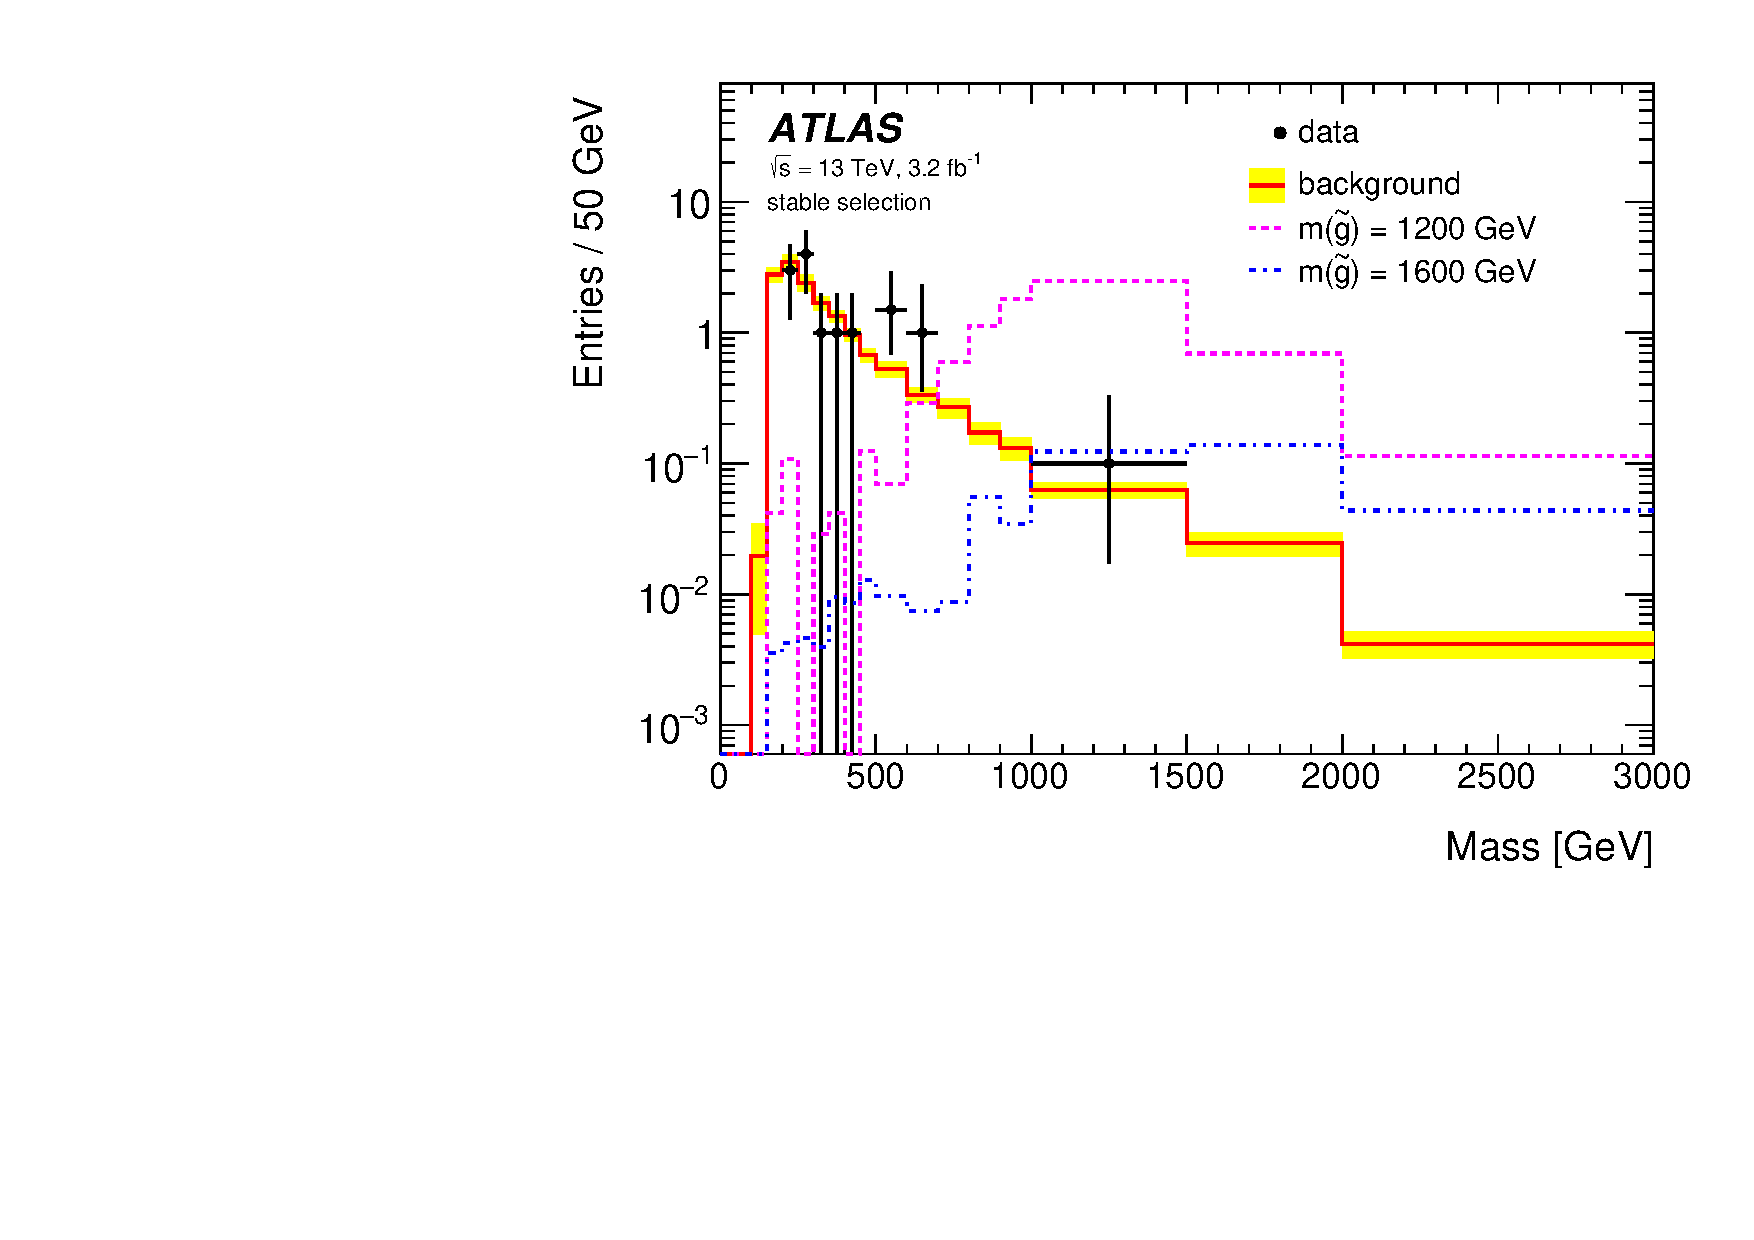
\includegraphics[width=\halffig]{figures/sr_mass_stable.pdf}
}
\subfloat{
  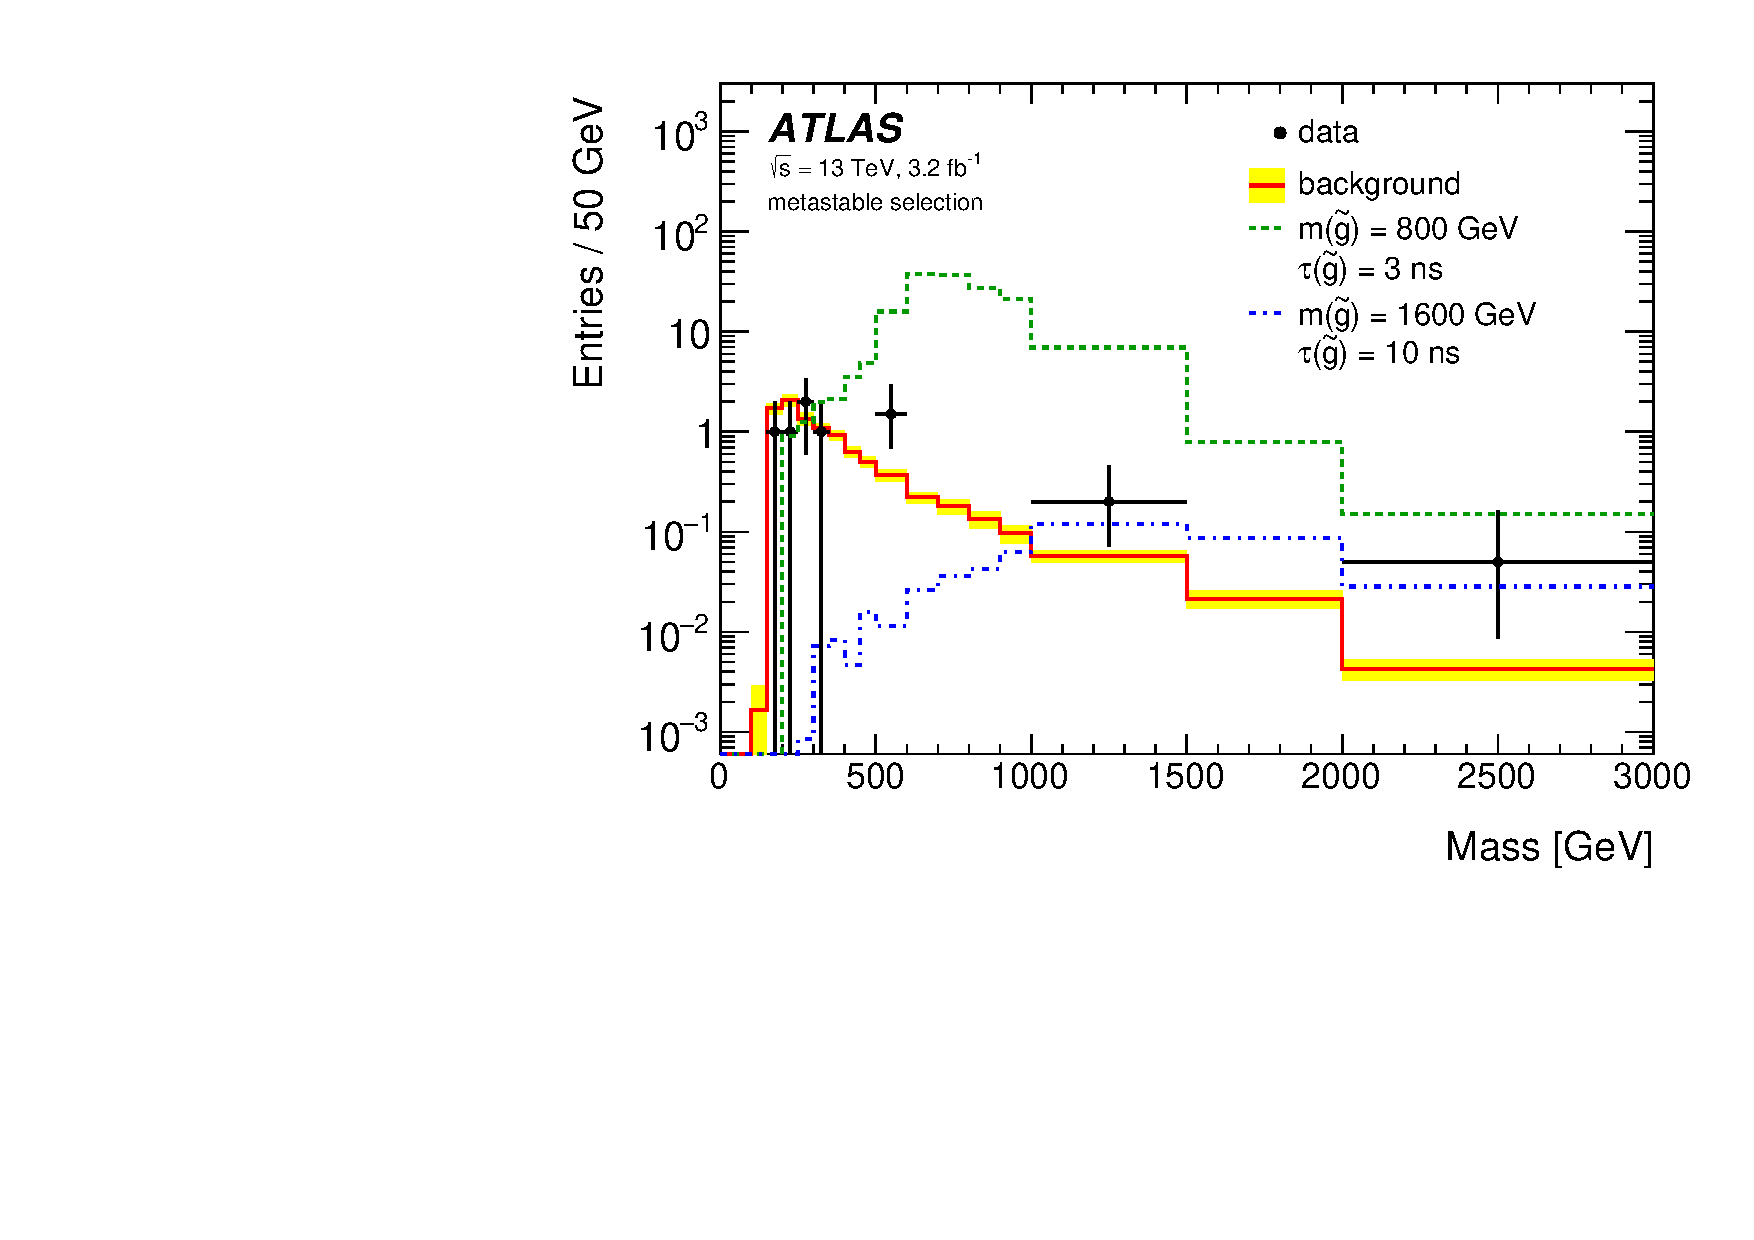
\includegraphics[width=\halffig]{figures/sr_mass_metastable.pdf}
}
\caption{The observed mass distribution of events in data and the generated background distribution in (a) the stable and (b) the metastable signal region. A few example simulated signal distributions are superimposed.}
\label{fig:signal_mass}
\end{figure}

% ----------------------------------------

\section{Cross Sectional Limits}

Because there is no observed significant excess of events in the signal region, this analysis sets upper limits on the allowed cross section for \rhadron production.
These limits are set for each mass point by counting the observed events in data, along with the expected background and simulated signal events, in windows of mass.
The mass windows are formed by fitting the distribution of signal events to a Gaussian distribution, and the window is then $\pm 1.4\sigma$ around the center of that Gaussian.
Two examples of the windows formed by this procedure are shown in Tables~\ref{tab:window_10ns}-\ref{tab:window_stable}, for the stable and 10 ns working points.
The corresponding counts of observed data, expected background, and simulated signal for those same working points are shown in Tables~\ref{tab:counts_stable}-\ref{tab:counts_10ns}.
Appendix~\ref{app:yields} includes the mass windows and counts for all of the considered signal points.

\begin{table}[!htbp]
  \begin{center}
    \begin{tabular}{ccc}
        \hline
        $m(\tilde{g})$ [GeV]  & Left Extremum [GeV] & Right Extremum [GeV] \\
        \hline
        1000    & 655 & 1349 \\
        1100    & 734 & 1455 \\
        1200    & 712 & 1631 \\
        1300    & 792 & 1737 \\
        1400    & 717 & 1926 \\
        1500    & 815 & 2117 \\
        1600    & 824 & 2122 \\
        1700    & 900 & 2274 \\
        1800    & 919 & 2344 \\
        \hline
    \end{tabular}
  \end{center}
  \caption{The left and right extremum of the mass window for each generated mass point with a 10 ns lifetime.}
  \label{tab:window_10ns}
\end{table}

\begin{table}[!htbp]
  \begin{center}
    \begin{tabular}{ccc}
        \hline
        $m(\tilde{g})$ [GeV]  & Left Extremum [GeV] & Right Extremum [GeV] \\
        \hline
        800    & 627 & 1053 \\
        1000    & 726 & 1277 \\
        1200    & 857 & 1584 \\
        1400    & 924 & 1937 \\
        1600    & 993 & 2308 \\
        1800    & 1004 & 2554 \\
        \hline
    \end{tabular}
  \end{center}
  \caption{The left and right extremum of the mass window used for each generated stable mass point.}
  \label{tab:window_stable}
\end{table}

\begin{table}[!htbp]
  \begin{center}
    \begin{tabular}{c|c|c|c}
      \hline
      $m(\tilde{g})$ [GeV]  & Expected Signal & Expected Background & Observed Data\\
      \hline
      800    & $462.83 \pm 14.86 $ & $1.764 \pm 0.080 $ & $2.0$ \\
      1000   & $108.73 \pm 3.38 $  & $1.458 \pm 0.070 $ & $1.0$ \\
      1200   & $31.74 \pm 0.95 $   & $1.137 \pm 0.060 $ & $1.0$ \\
      1400   & $10.22 \pm 0.29 $   & $1.058 \pm 0.058 $ & $1.0$ \\
      1600   & $3.07 \pm 0.09 $    & $0.947 \pm 0.054 $ & $1.0$ \\
      1800   & $1.08 \pm 0.05 $    & $0.940 \pm 0.054 $ & $1.0$ \\
      \hline
    \end{tabular}
  \end{center} 
  \caption{The expected number of signal events, the expected number of background events, and the observed number of events in data with their respective statistical errors within the respective mass window for each generated stable mass point}
  \label{tab:counts_stable}
\end{table}

\begin{table}[!htbp]
  \begin{center}
    \begin{tabular}{cccc}
      \hline
      $m(\tilde{g})$ [GeV]  & Expected Signal & Expected Background & Observed Data\\ 
      \hline
      1000    & $144.48 \pm 5.14 $ & $1.499 \pm 0.069 $ & $2.0$ \\
      1100    & $73.19 \pm 2.61 $  & $1.260 \pm 0.060 $ & $2.0$ \\
      1200    & $41.54 \pm 1.41 $  & $1.456 \pm 0.067 $ & $2.0$ \\
      1300    & $22.58 \pm 0.77 $  & $1.201 \pm 0.058 $ & $2.0$ \\
      1400    & $12.70 \pm 0.42 $  & $1.558 \pm 0.071 $ & $2.0$ \\
      1500    & $6.73 \pm 0.24 $   & $1.237 \pm 0.060 $ & $2.0$ \\
      1600    & $3.90 \pm 0.13 $   & $1.201 \pm 0.058 $ & $2.0$ \\
      1700    & $2.27 \pm 0.07 $   & $1.027 \pm 0.052 $ & $2.0$ \\
      1800    & $1.34 \pm 0.04 $   & $1.019 \pm 0.052 $ & $2.0$ \\
      \hline
    \end{tabular}
  \end{center}
  \caption{The expected number of signal events, the expected number of background events, and the observed number of events in data with their respective statistical errors within the respective mass window for each generated mass point with a lifetime of 10 ns.}
  \label{tab:counts_10ns}
\end{table}


The 95\% confidence level upper limits on the cross sections for a large grid of masses (between 800 and 1800 \GeV) and lifetimes (between 0.4 and stable) are extracted from these counts with the $CL_{S}$ method using the profile likelihood ratio as a test statistic~\cite{CLS_method}.
For this procedure, the systematic uncertainties estimated for the signal and background yields are treated as Gaussian-distributed nuissance parameters.
The uncertainty on the normalization of the expected background distribution is included in the expected background events.
At this point the expected cross section limit is calculated for both the metastable and stable signal region for each lifetime point, and the region with the best expected limit is selected for each lifetime.
Using that procedure, the metastable region is used for lifetimes up to and including 30 ns, and the stable region for lifetimes above it. 


The resulting cross-sectional upper limits are shown as a function of mass in Figure~\ref{fig:xsec_limit_stable} and Figure~\ref{fig:xsec_limit_metastable} for each lifetime considered.
The limits are interpolated linearly between each mass point, and the dependence of the limit on the mass is small as the efficiency is relatively constant for large \rhadron masses.
There is however a strong dependence on lifetime, as discussed in Section~\ref{sec:efficiency}, where the probability to form a fully reconstructed track and the kinematic freedom to produce \met result in a local maximum in the limit at 10-30 ns.
The figures also include the expected cross section for pair-produced gluino \rhadrons for reference.
For the 10 ns and stable cross section limits, both the observed limit and expected cross section for the Run 1, 8 \TeV version of this analysis are included.
There the cross sectional limits are lower because of the increased available luminosity, while the signal cross sections were also much lower because of the lower collision energy.

\begin{figure}
\centering
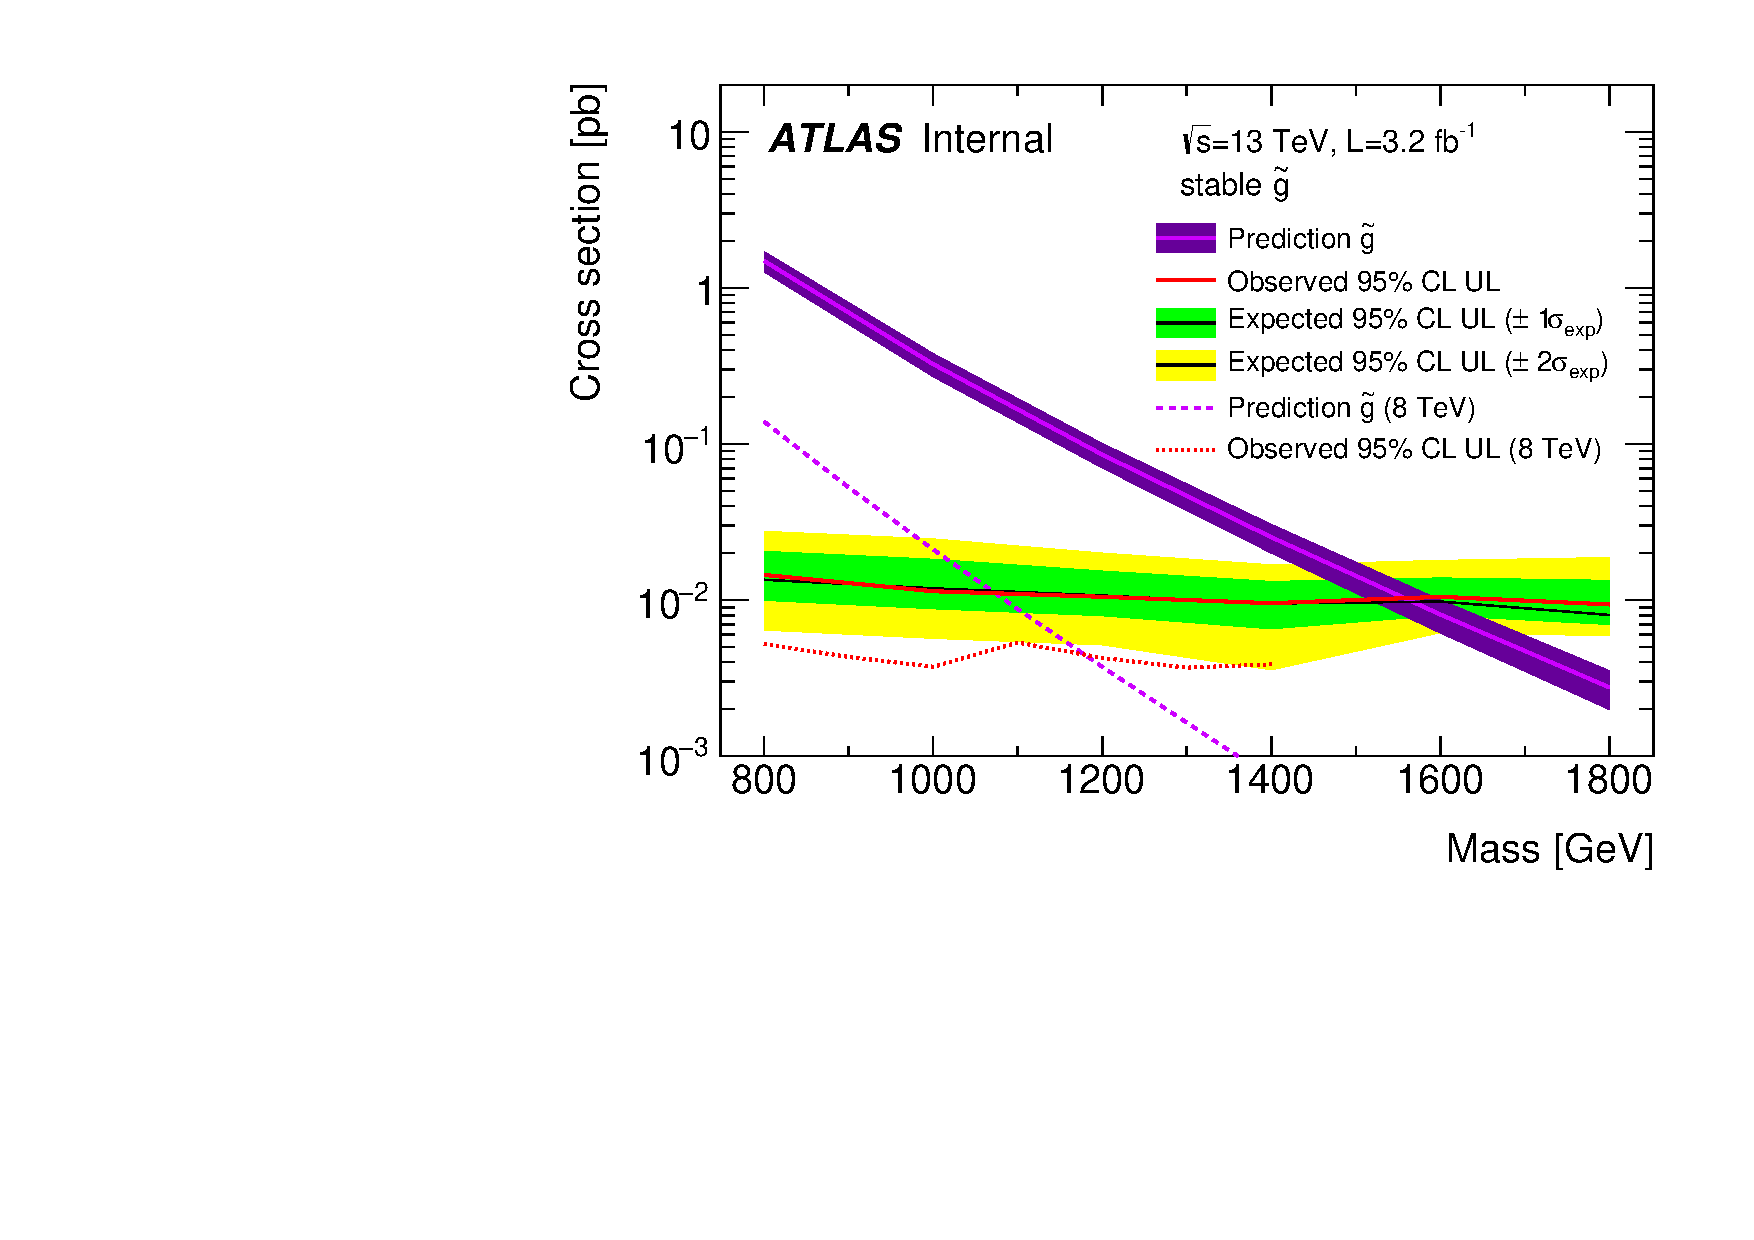
\includegraphics[width=\fullfig]{figures/xsec_limit_stable.pdf}
\caption{The observed and expected cross section limits as a function of mass for the stable simulated signal. The predicted cross section values for the corresponding signals are included.}
\label{fig:xsec_limit_stable}
\end{figure}

\begin{figure}
\subfloat{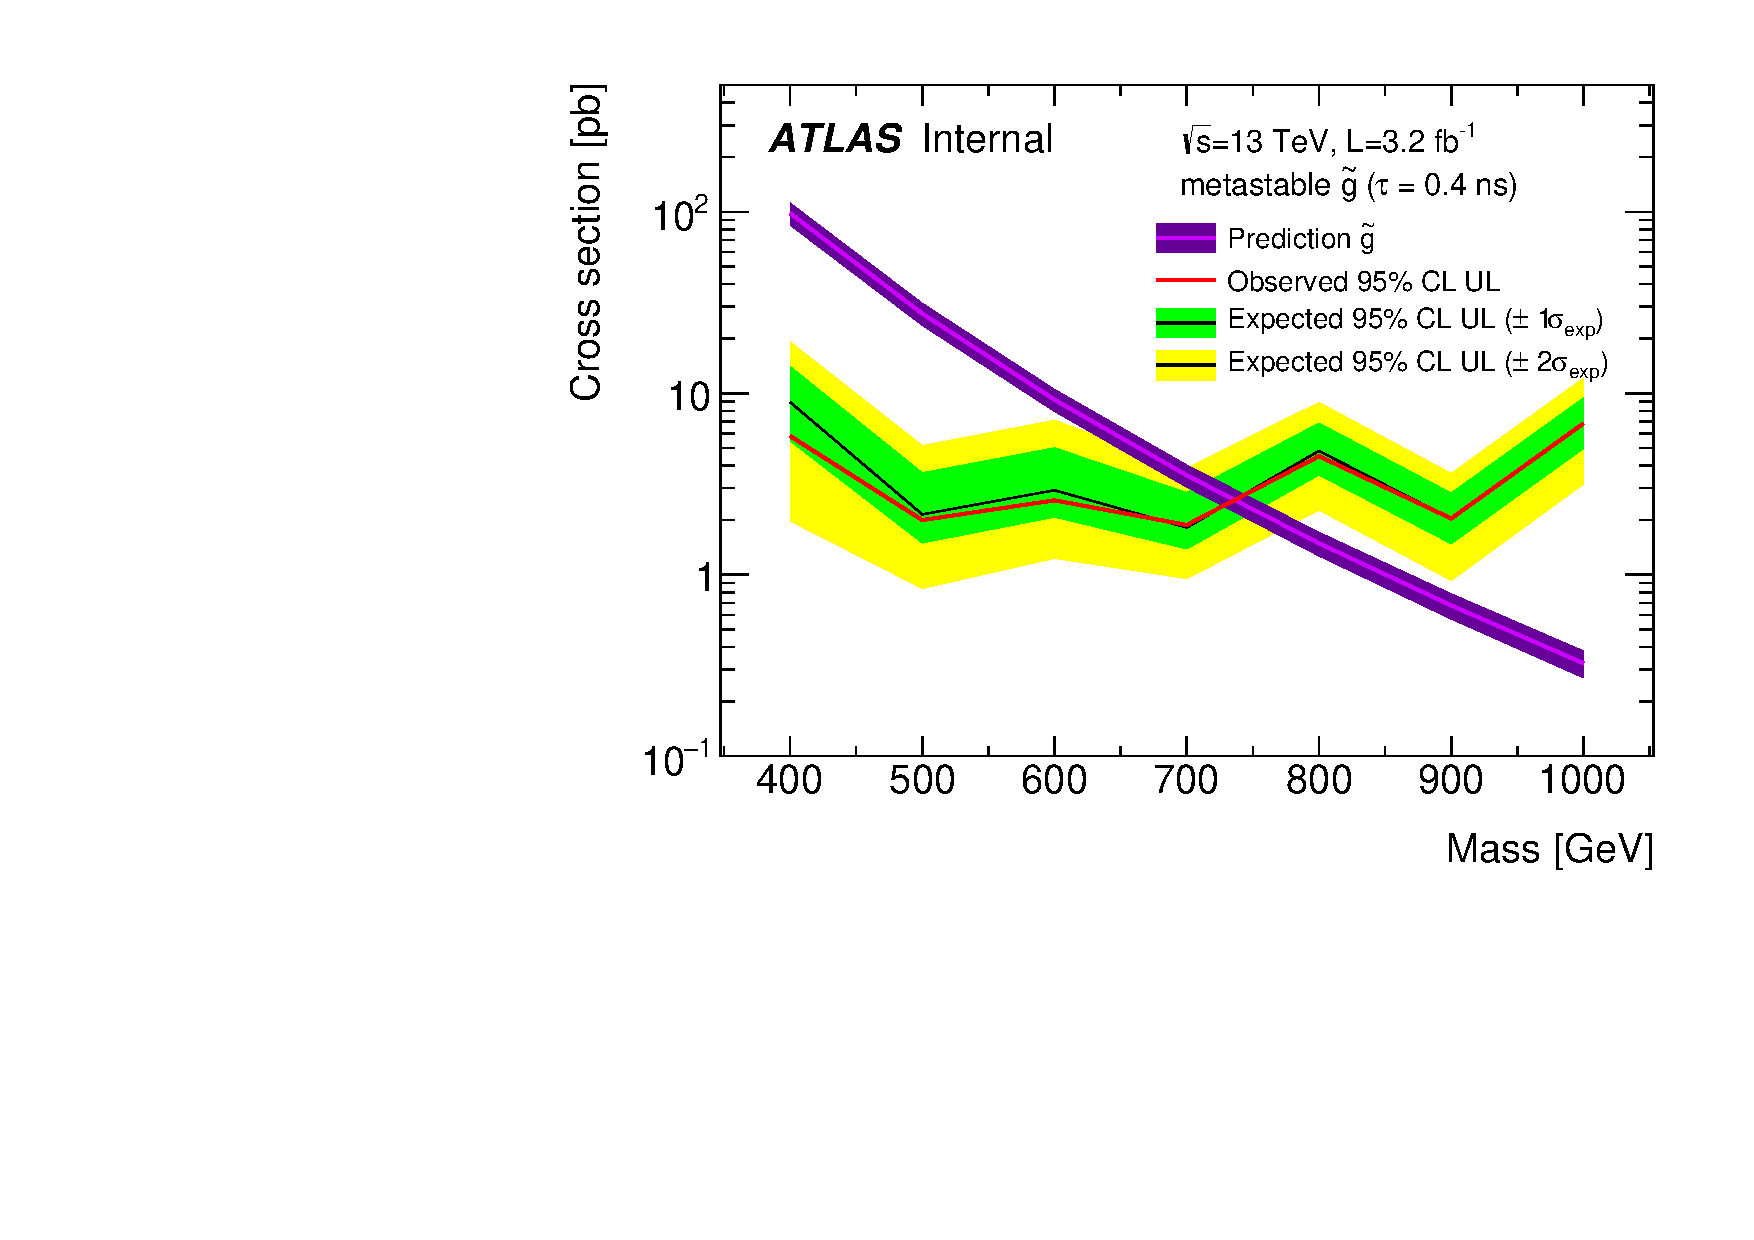
\includegraphics[width=\halffig]{figures/xsec_limit_p4ns.pdf}}
\subfloat{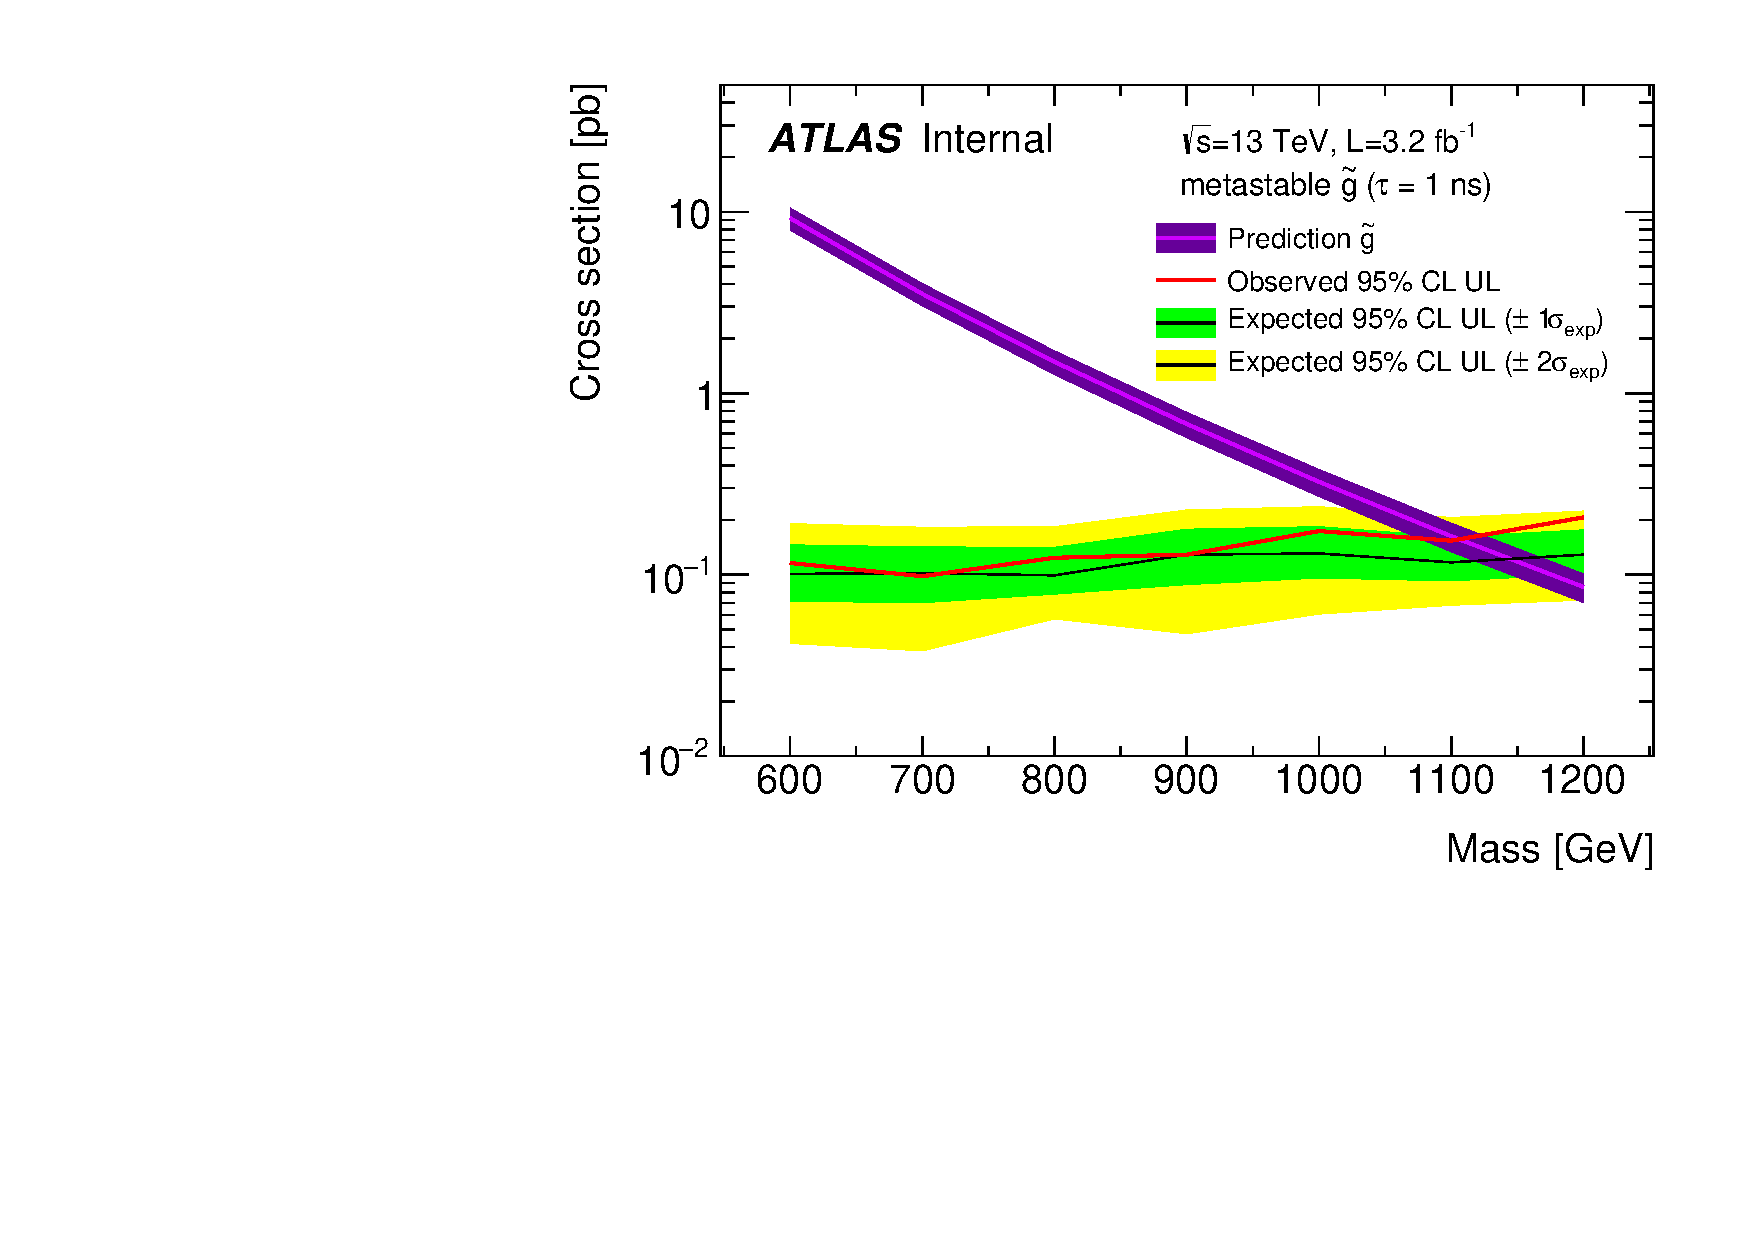
\includegraphics[width=\halffig]{figures/xsec_limit_1ns.pdf}}\\
\subfloat{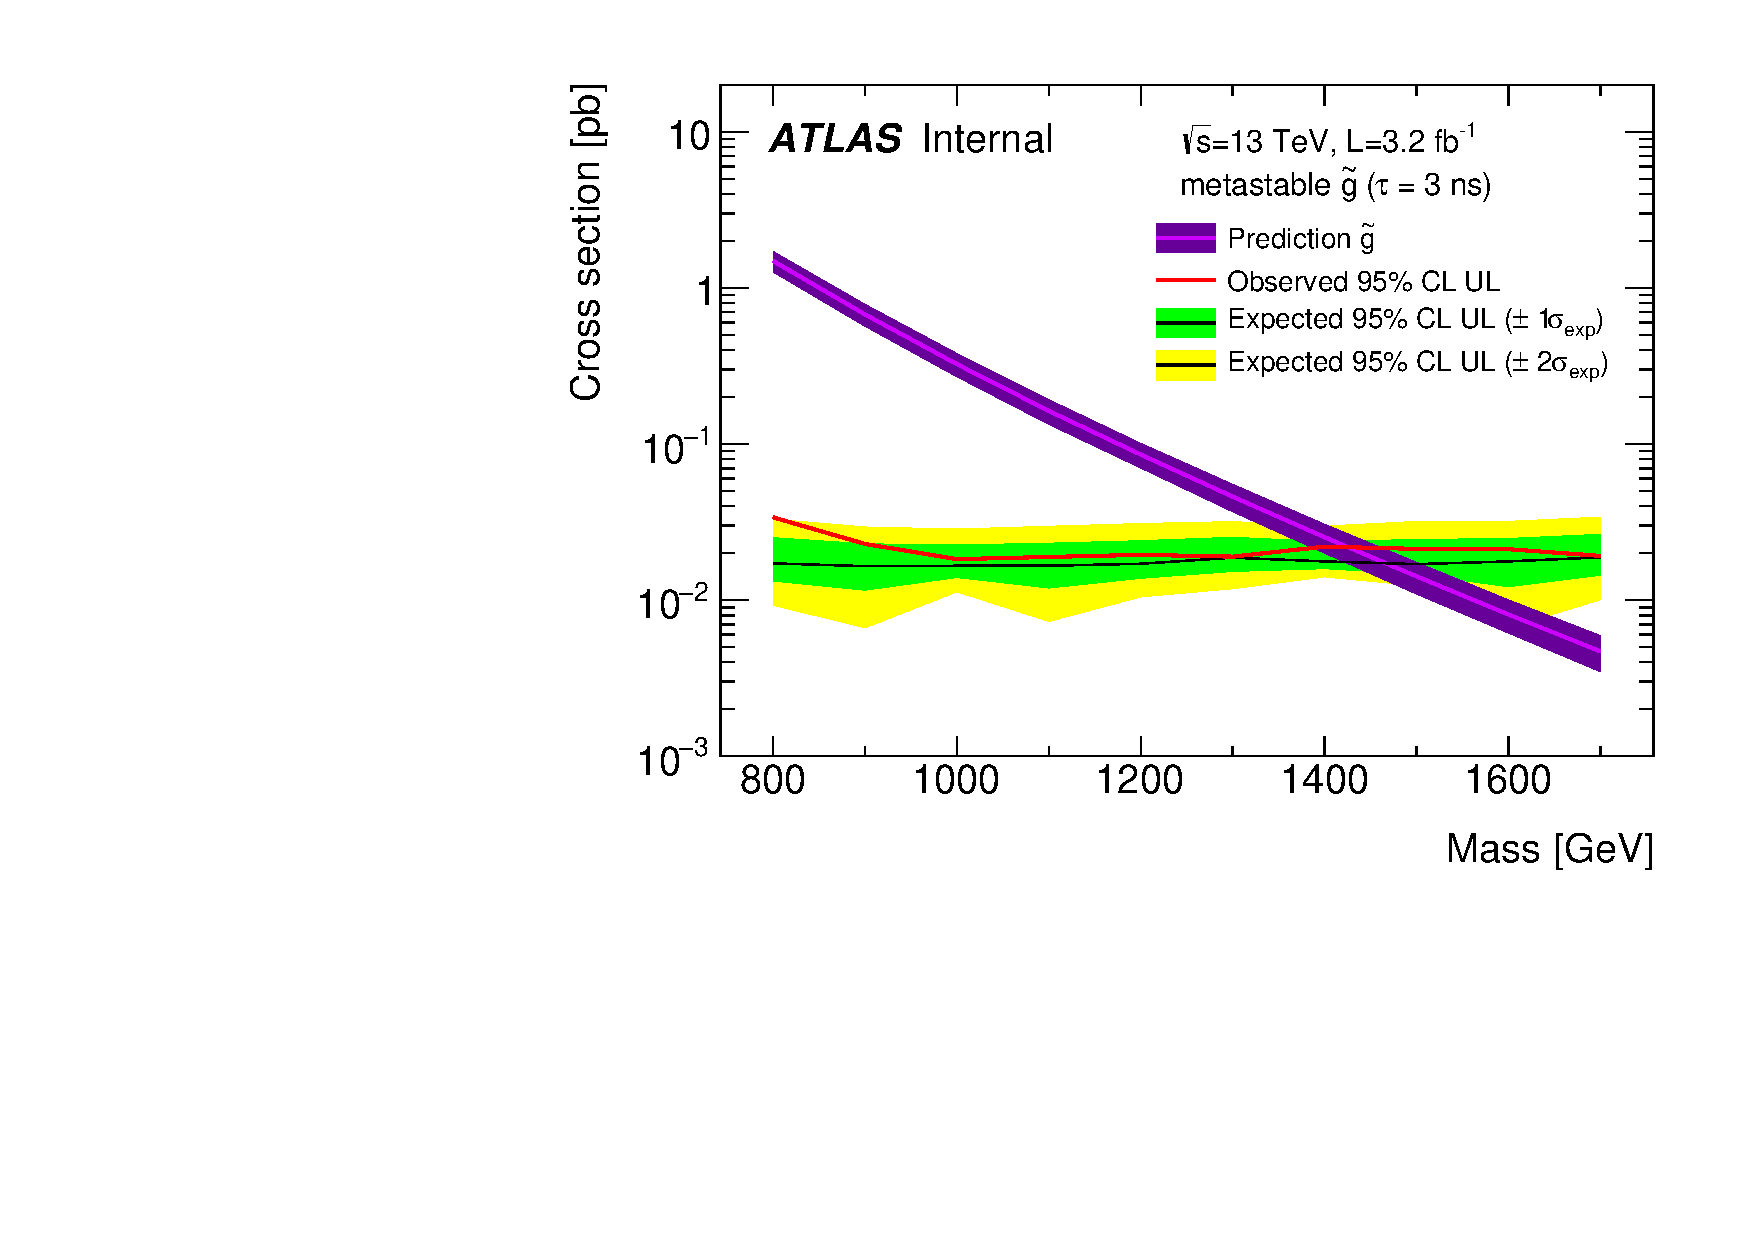
\includegraphics[width=\halffig]{figures/xsec_limit_3ns.pdf}}
\subfloat{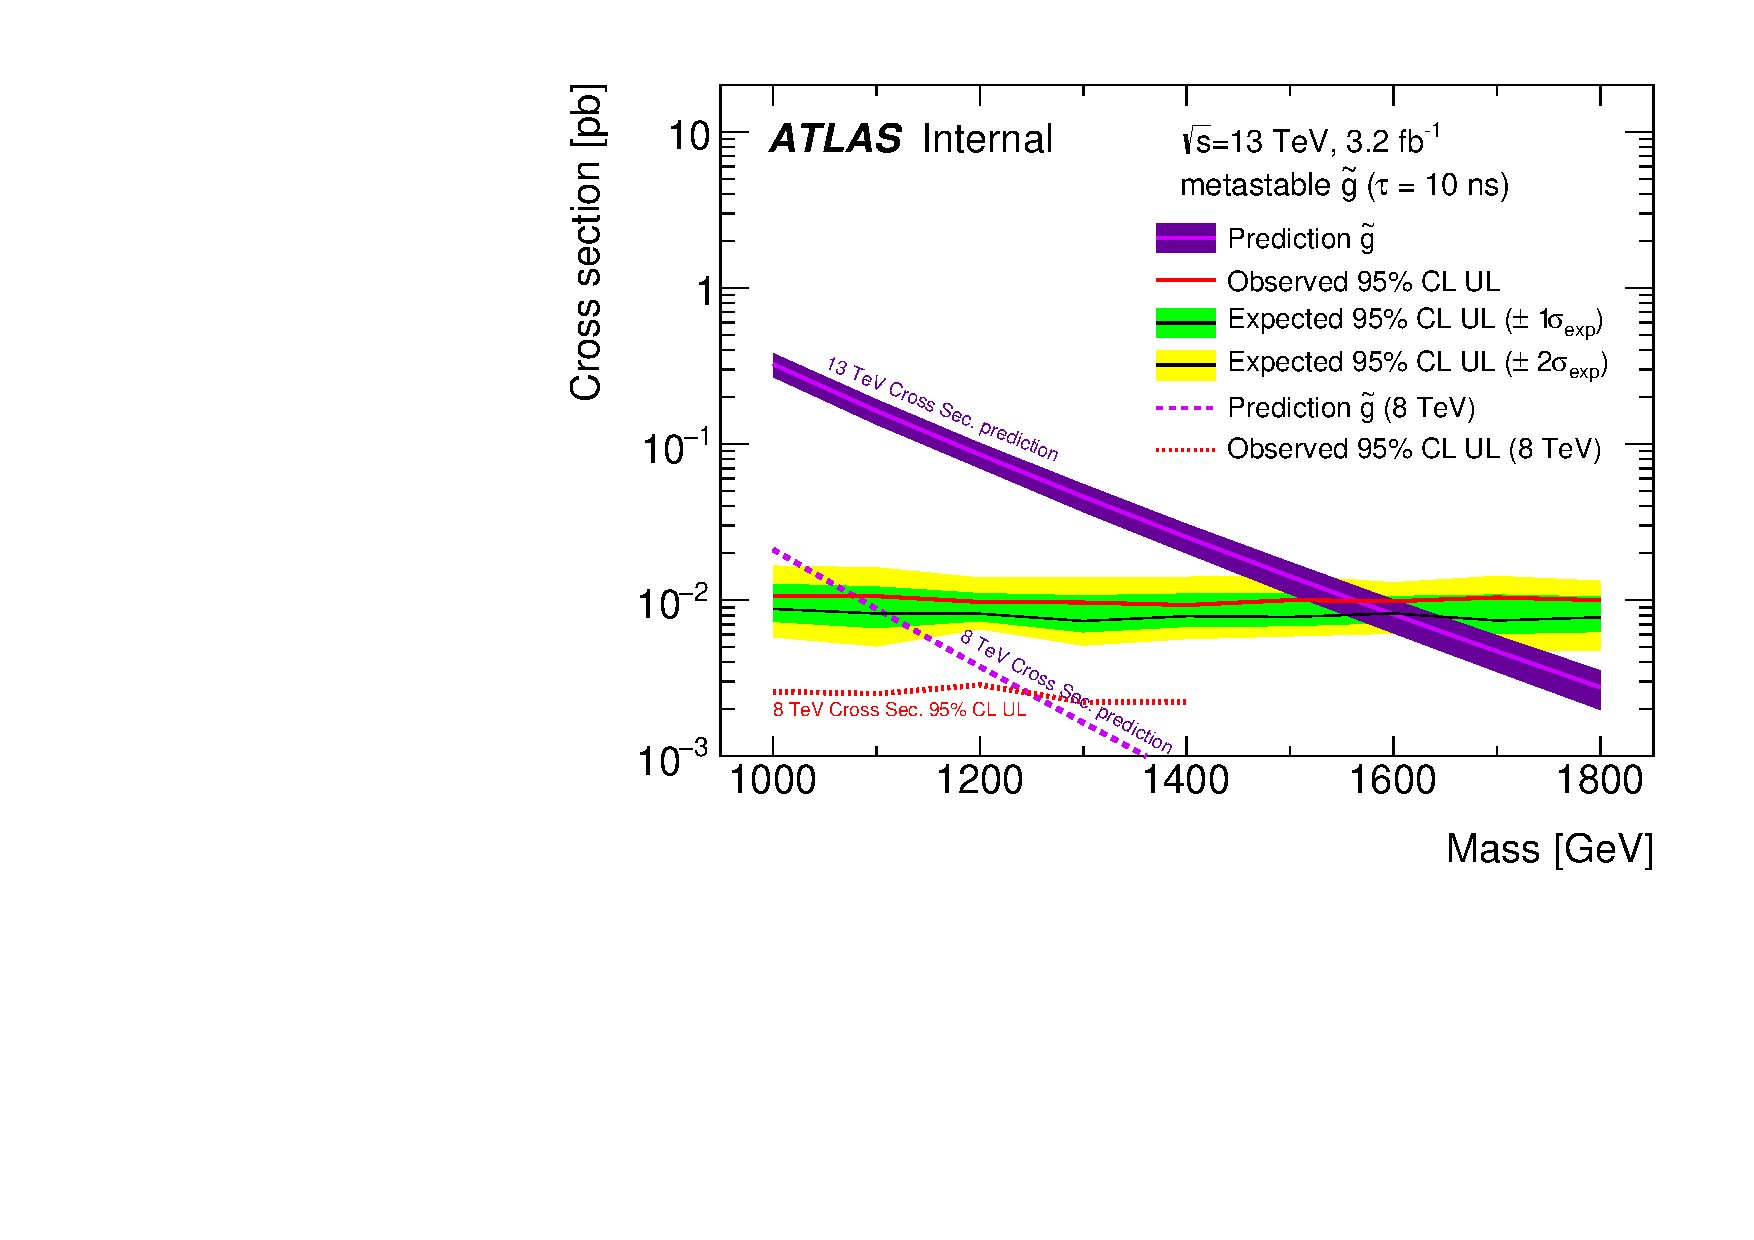
\includegraphics[width=\halffig]{figures/xsec_limit_10ns.pdf}}\\
\subfloat{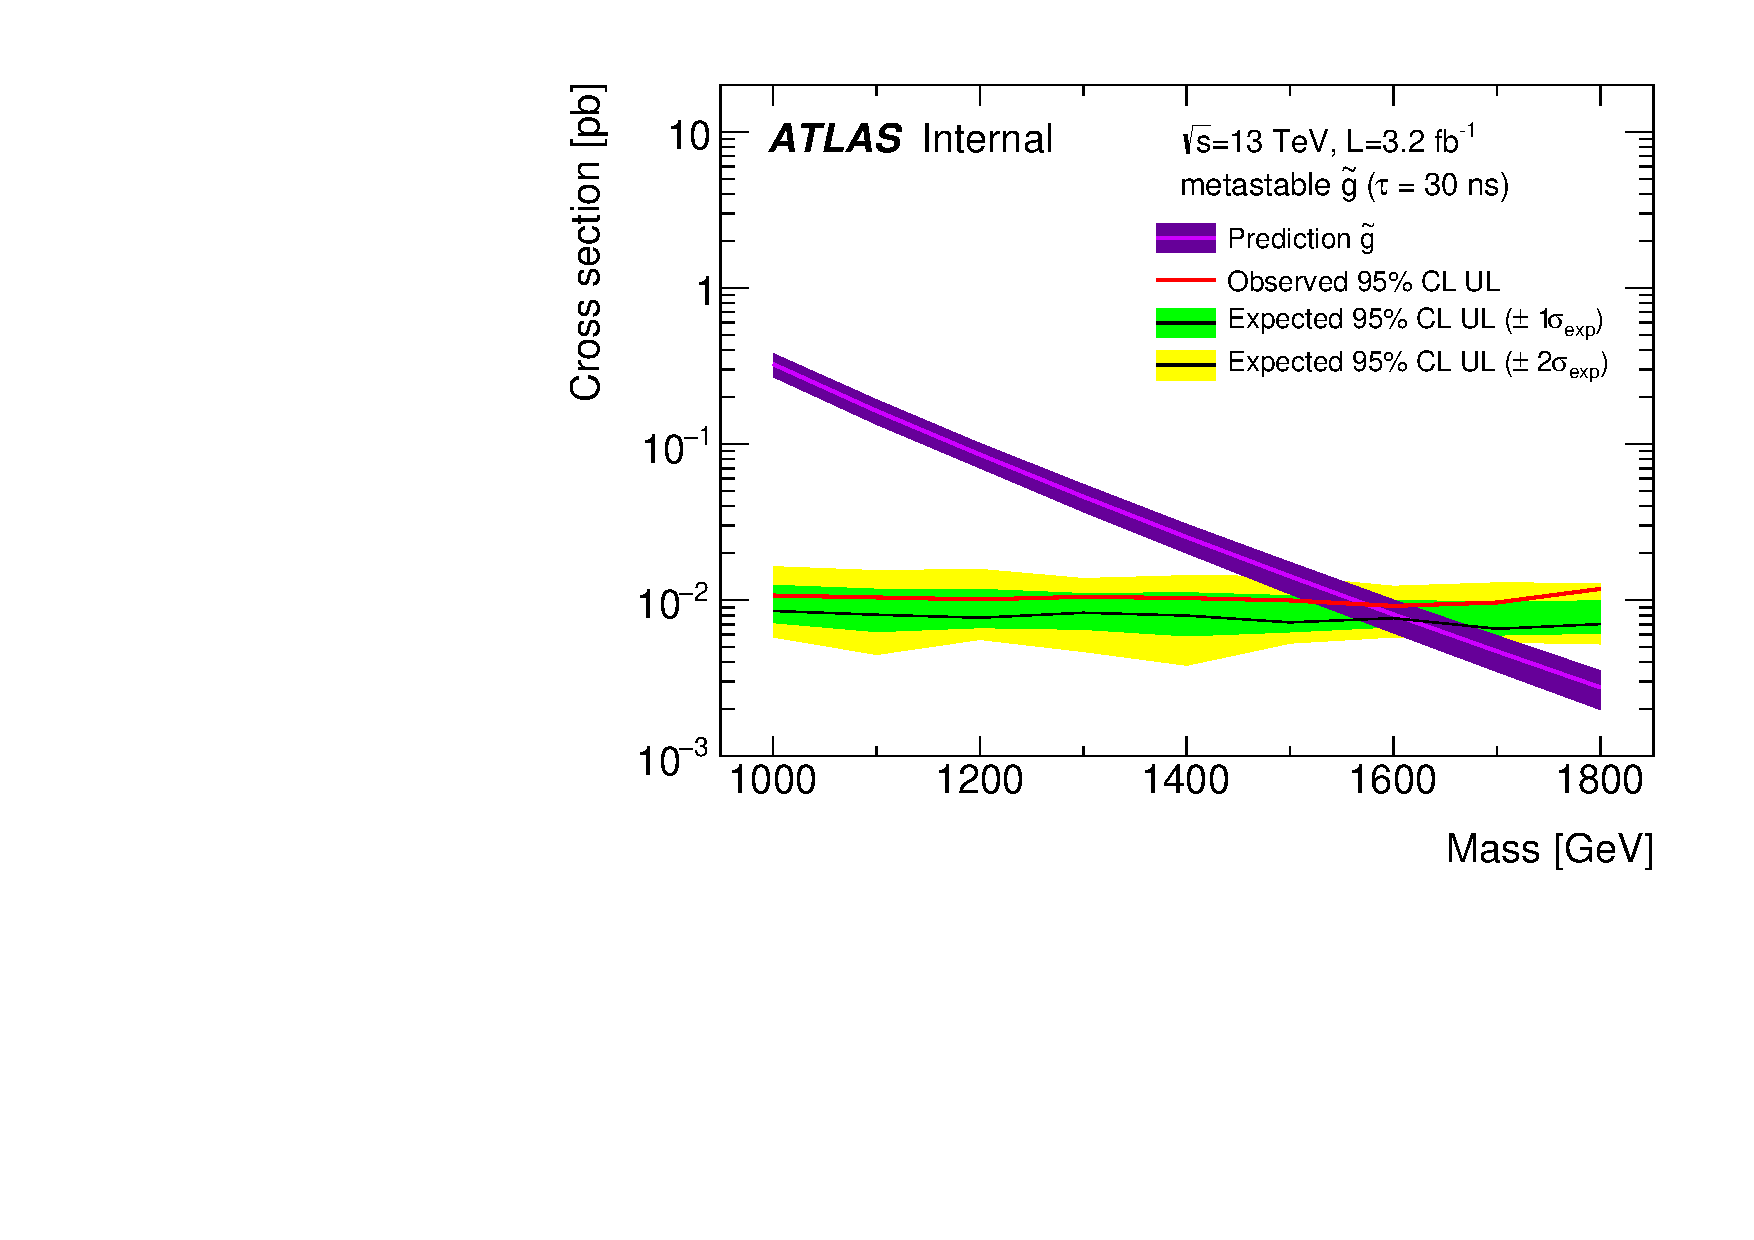
\includegraphics[width=\halffig]{figures/xsec_limit_30ns.pdf}}
\subfloat{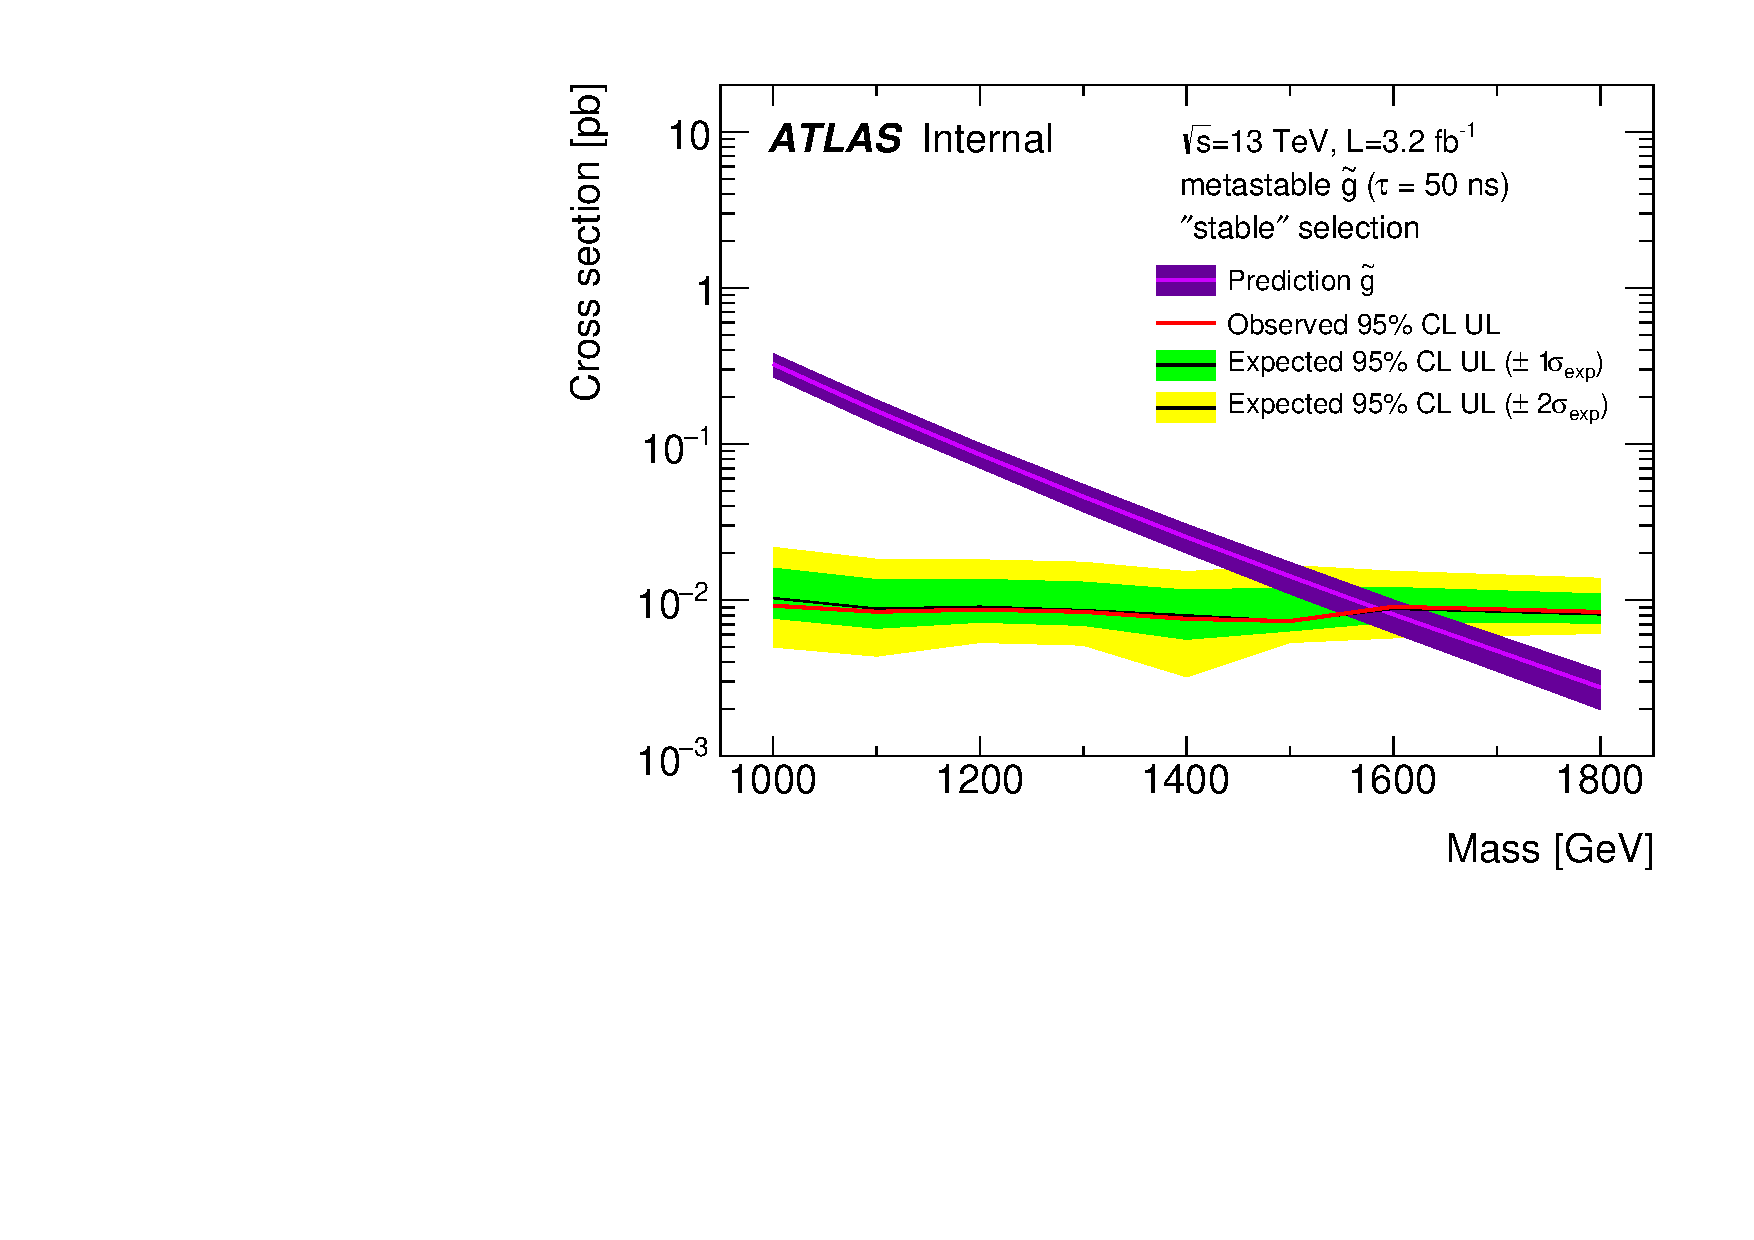
\includegraphics[width=\halffig]{figures/xsec_limit_50ns.pdf}}\\
\caption{The observed and expected cross section limits as a function of mass for each generated lifetime. The predicted cross section values for the corresponding signals are included.}
\label{fig:xsec_limit_metastable}
\end{figure}



% ----------------------------------------

\section{Mass Limits}

The cross-sectional limits can then be used to derive a lower mass limit for gluino \rhadrons by comparing them to the theoretically predicted production cross sections.
These mass limits range from only 740 \GeV at the lowest lifetimes considered, where the selection efficiency is very low, to up to 1580 \GeV at 30 ns where the selection efficiency is maximized.
The observed and expected mass limits for each lifetime point are detailed in Table~\ref{tab:mass_limits}, which also lists which selection region was used for each lifetime.
These excluded range of masses as a function of lifetime is also shown in Figure~\ref{fig:mass_limits}.
The Run 1 limits are included for comparison; the limits have increased by about 200 \GeV on average.
The search has also improved since the previous incarnation from Run 1 in optimizing the region between 30 \GeV and detector-stable lifetimes by introducing the second signal region.
The definition of the stable region prevents the significant drop in mass limit that occurred above 30 \GeV in the Run 1 analysis.

\begin{table}[htp]
\centering
\begin{tabular}{cccc}
  \hline
  Selection & $\tau$ [ns] & $M_{\mathrm{obs}}>$[\GeV] & $M_{\mathrm{exp}}>$[\GeV] \\
  \hline
  Metastable   & 0.4       & 740       & 730 \\
          "   & 1.0       & 1110       & 1150 \\
          "   & 3.0       & 1430       & 1470\\
          "   & 10        & 1570       & 1600 \\
          "   & 30        & 1580      & 1620 \\
  \hline
  Stable       & 50         & 1590      & 1590 \\
      "        & stable           & 1570     & 1580 \\
  \hline
\end{tabular}
\caption{The observed and expected 95\% CL lower limit on mass for gluino~\rhadrons for each considered lifetime.}
\label{tab:mass_limits}
\end{table}%

\begin{figure}[htbp]
\centering
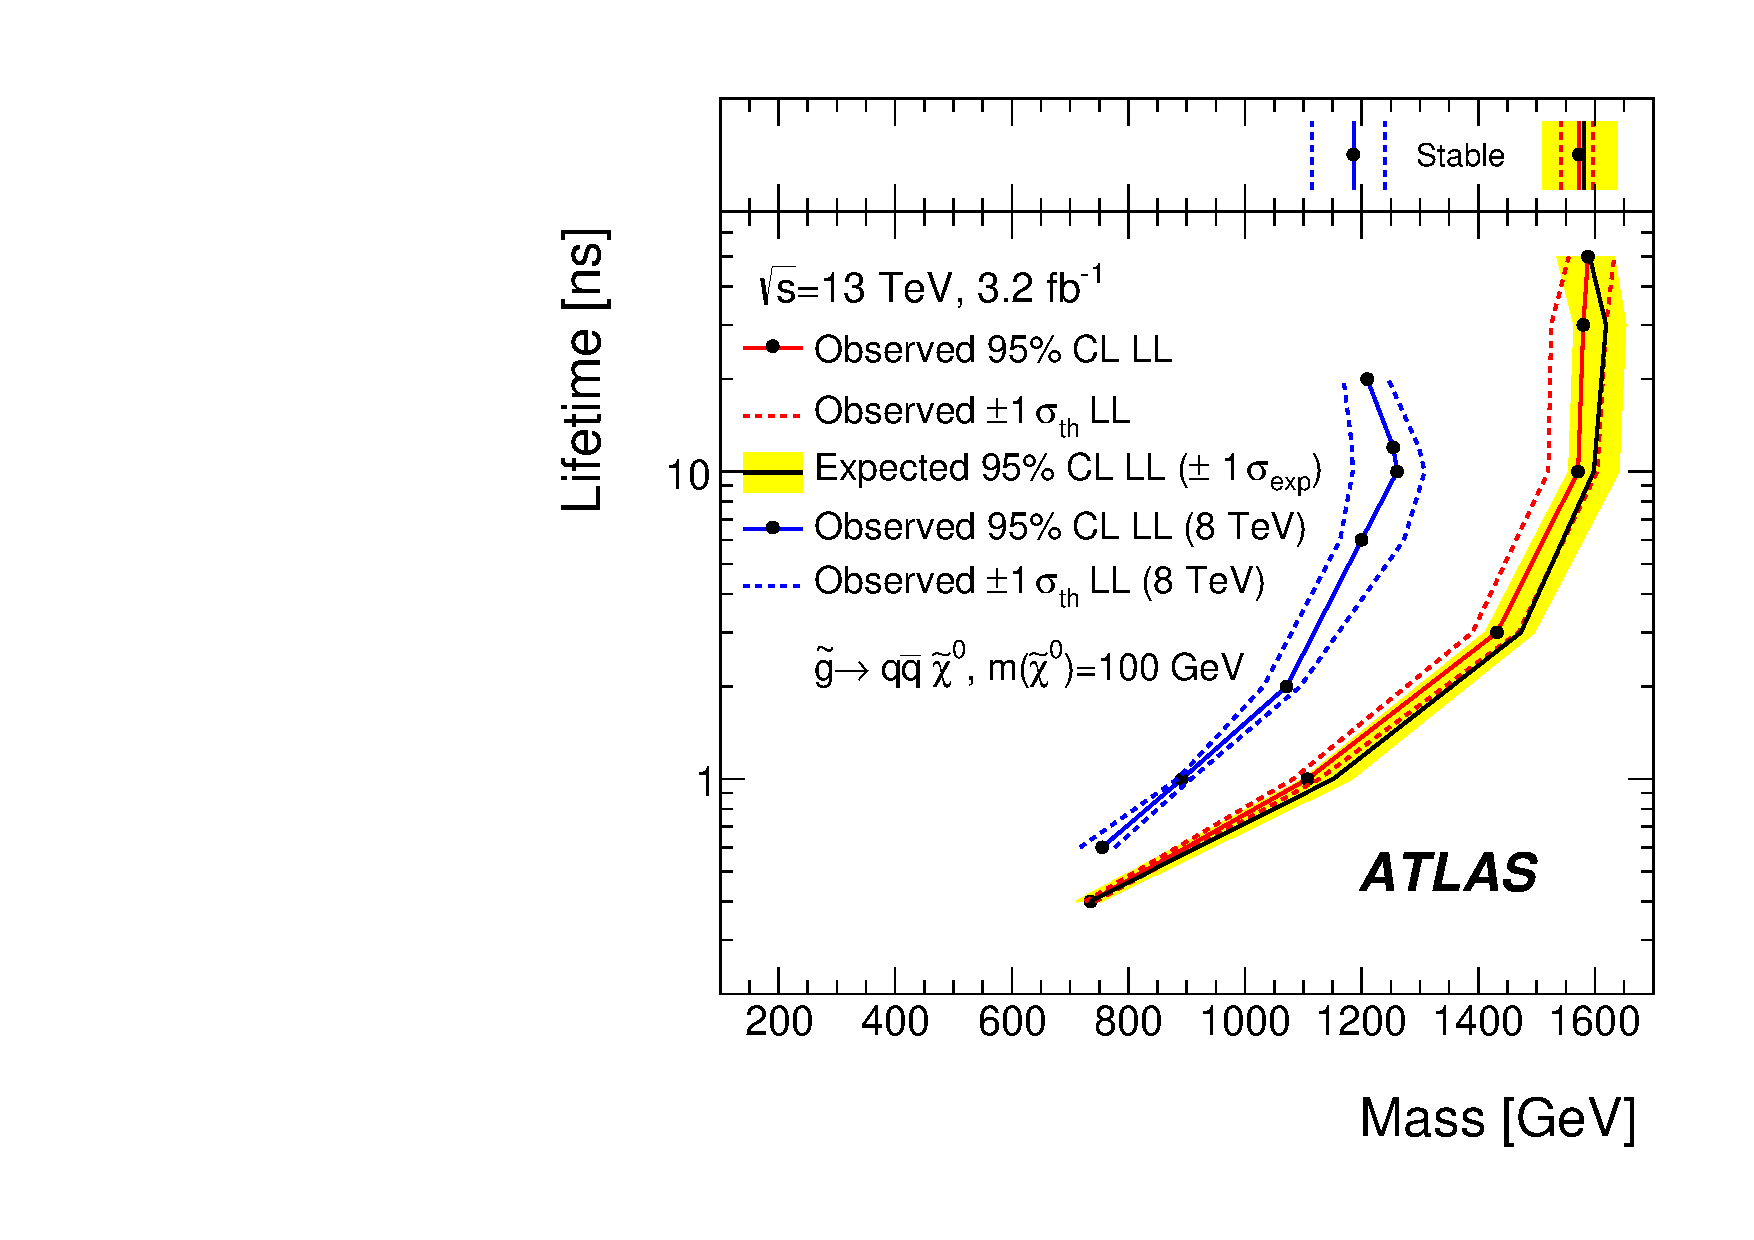
\includegraphics[width=\fullfig]{figures/taumass_exclusion.pdf}  
\caption{The excluded range of masses as a function of gluino lifetime. The expected lower limit (LL), with its experimental $\pm 1 \sigma$ band, is given with respect to the nominal theoretical cross-section. The observed 95\% LL obtained at $\sqrt{s} = 8$~\TeV~\cite{SUSY-2014-09} is also shown for comparison.}
\label{fig:mass_limits}
\end{figure}

% ----------------------------------------

\section{Context for Long-Lived Searches}
This search plays an important role in the current, combined ATLAS search for long lived particles.
The mass limits provided by various ATLAS searches for long-lived gluino \rhadrons can be seen in Figure~\ref{fig:combined_rhadrons}.
This search provides the most competitive limit for lifetimes between 3 ns up through very long lifetimes, where it is still competitive with dedicated searches for stable particles.
The limits placed on gluino production are very similar to the limits on promptly decaying models.

\begin{figure}[htbp]
\centering
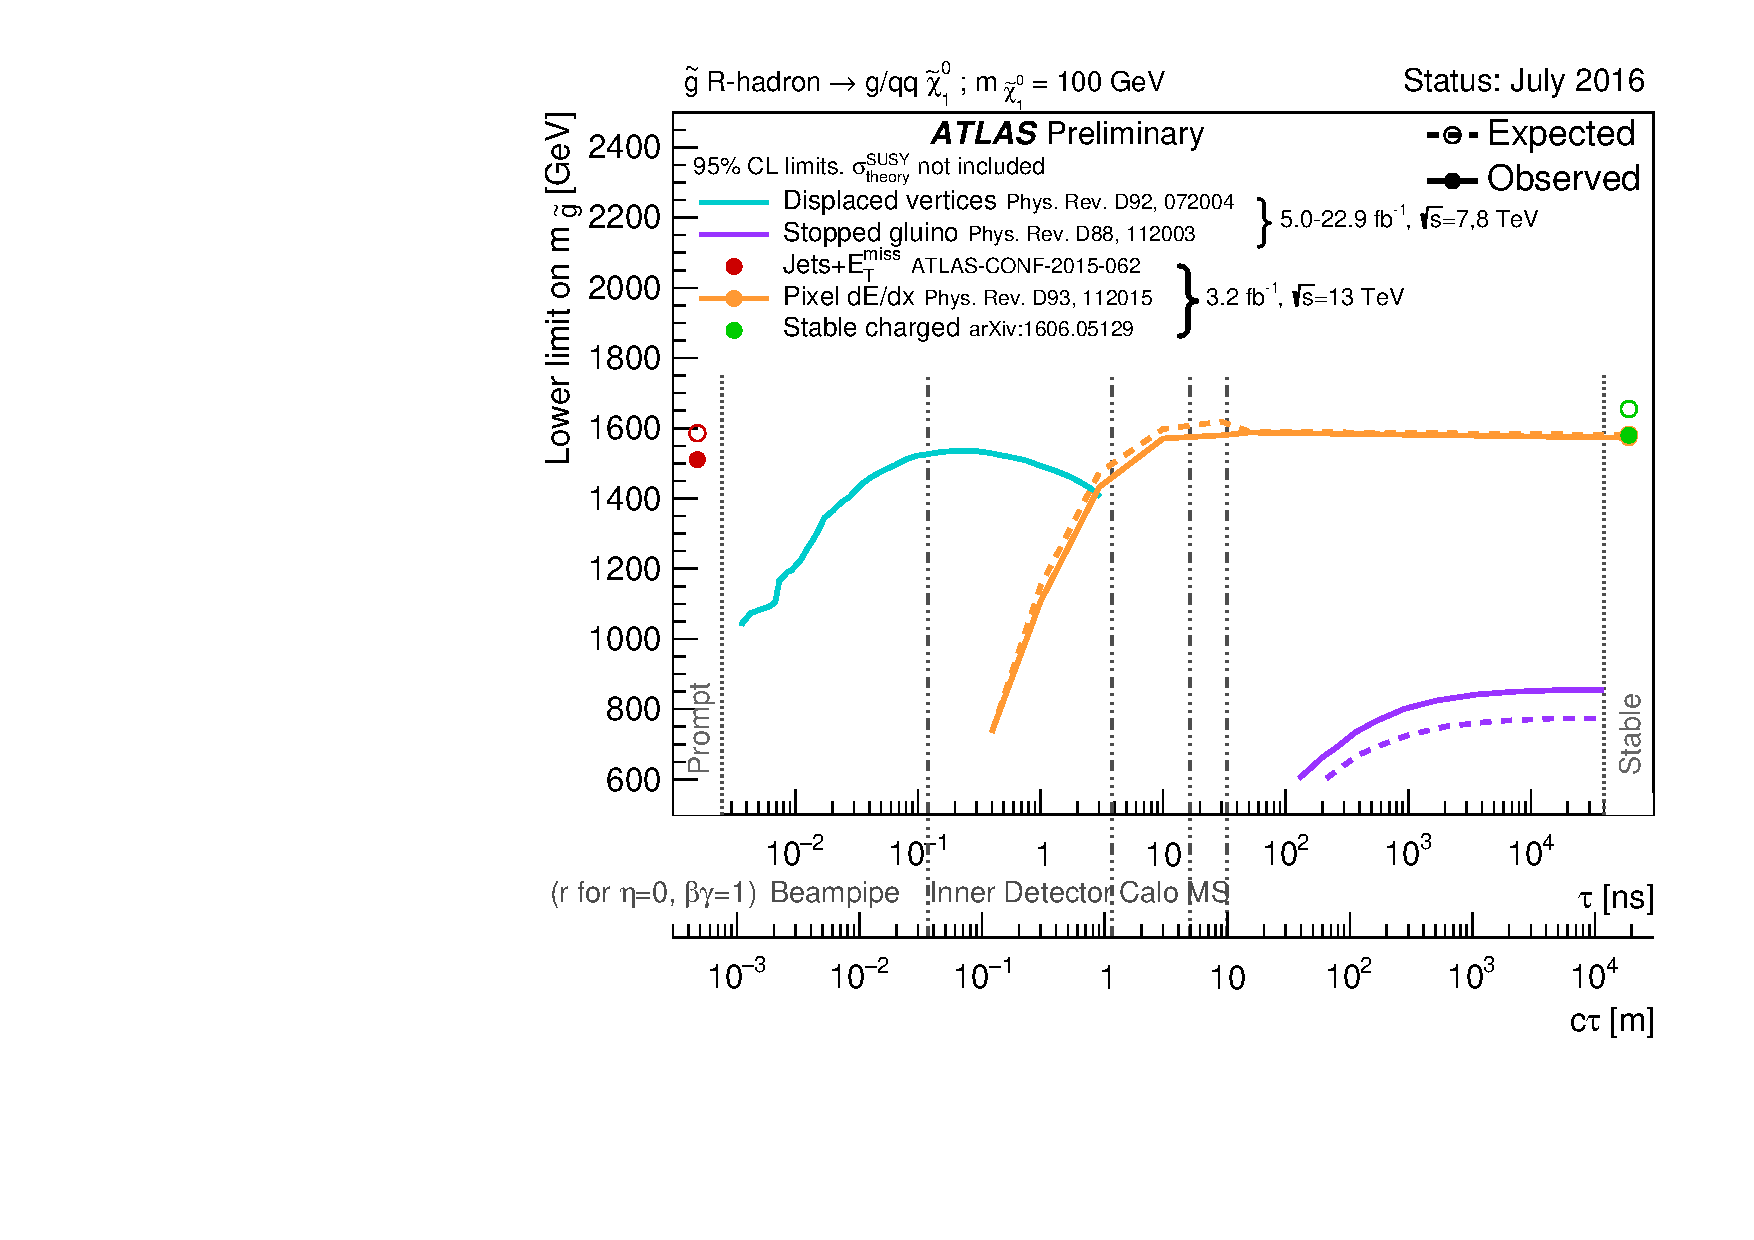
\includegraphics[width=\fullfig]{figures/combined_rhadrons.pdf}  
\caption{The constraints on the gluino mass as a function of lifetime for a split-supersymmetry model with the gluino \rhadrons decaying into a gluon or light quarks and a neutralino with mass of 100 GeV. The solid lines indicate the observed limits, while the dashed lines indicate the expected limits. The area below the curves is excluded. The dots represent results for which the particle is assumed to be prompt or stable.}
\label{fig:combined_rhadrons}
\end{figure}


% ----------------------------------------
